% ============================================================
% Capítulo 3 — Fundamentos de topología computacional
% Requiere: amsmath, amssymb, amsthm, tikz, booktabs
% Entornos: definicion, teorema, proposicion, lema,
%           ejemplo, observacion (definir en el preámbulo)
% Bibliografía: refs.bib
% ============================================================

\chapter{Fundamentos de topología computacional}
\label{cap:fundamentos}

Segmentar bien no consiste solo en acertar píxel a píxel: un objeto partido
en dos o unido a otro mediante un puente espurio apenas penaliza una métrica
de solapamiento, pero altera la \emph{forma} del objeto segmentado. Este
capítulo, núcleo teórico del trabajo, reúne las herramientas
matemáticas que permiten cuantificar esa forma. Seguimos principalmente a
Edelsbrunner y Harer~\cite{edelsbrunner2010}: los complejos
(Sección~\ref{sec:complejos}), la homología
(Sección~\ref{sec:homologia}) y la homología persistente
(Sección~\ref{sec:persistencia}). Después introducimos las distancias entre
diagramas de persistencia (Sección~\ref{sec:distancias}) y, por último,
describimos cómo estas ideas se convierten en métricas y funciones de
pérdida para segmentación (Sección~\ref{sec:topo-segmentacion}), con
especial atención a \emph{Betti matching}~\cite{stucki2023} y
\emph{Topograph}~\cite{lux2025}.

Trabajamos siempre con coeficientes en el cuerpo $\mathbb{F}_2=\{0,1\}$,
donde $1+1=0$. Esta elección simplifica los cálculos (no hay signos ni
orientaciones) y es la habitual en topología computacional.

% ------------------------------------------------------------
\section{Complejos}
\label{sec:complejos}
% ------------------------------------------------------------

Para calcular invariantes topológicos con un ordenador necesitamos
representar los espacios de forma finita y combinatoria. Los complejos
simpliciales son la representación clásica; los complejos cúbicos son la
adaptada a imágenes.

\subsection{Complejos simpliciales}

Sean $u_0,\dots,u_p\in\mathbb{R}^d$ puntos afínmente independientes, es
decir, tales que los vectores $u_i-u_0$, $1\le i\le p$, son linealmente
independientes.

\begin{definicion}[{\cite[§III.1]{edelsbrunner2010}}]
Un \emph{$p$-símplice} es la envolvente convexa
$\sigma=\operatorname{conv}\{u_0,\dots,u_p\}$ de $p+1$ puntos afínmente
independientes; su \emph{dimensión} es $\dim\sigma=p$. Una \emph{cara} de
$\sigma$ es la envolvente convexa de un subconjunto no vacío de los $u_i$;
escribimos $\tau\le\sigma$.
\end{definicion}

Los símplices de dimensión $0,1,2$ y $3$ son vértices, aristas, triángulos
y tetraedros.

\begin{figure}[ht]
\centering
\begin{minipage}[c]{0.4\textwidth}
\centering
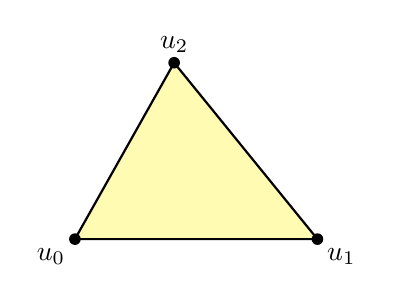
\begin{tikzpicture}[scale=1.4]
  \fill[yellow!30] (0,0) -- (2.2,0) -- (0.9,1.6) -- cycle;
  \draw[thick] (0,0) -- (2.2,0) -- (0.9,1.6) -- cycle;
  \fill (0,0) circle (1.5pt) node[below left] {$u_0$};
  \fill (2.2,0) circle (1.5pt) node[below right] {$u_1$};
  \fill (0.9,1.6) circle (1.5pt) node[above] {$u_2$};
\end{tikzpicture}
\end{minipage}
\begin{minipage}[c]{0.55\textwidth}
Versión abstracta:
\[
  \bigl\{\{u_0\},\{u_1\},\{u_2\},\{u_0,u_1\},\{u_0,u_2\},\{u_1,u_2\},\{u_0,u_1,u_2\}\bigr\}
\]
\end{minipage}
\caption{Un 2-símplice geométrico (izquierda) y su versión abstracta, la familia de sus caras (derecha).}
\label{fig:simplice}
\end{figure}

\begin{definicion}[{\cite[§III.1]{edelsbrunner2010}}]
Un \emph{complejo simplicial} es una colección finita $K$ de símplices tal
que (i) si $\sigma\in K$ y $\tau\le\sigma$, entonces $\tau\in K$; y (ii) la
intersección de dos símplices de $K$ es vacía o una cara común de ambos.
Su \emph{espacio subyacente} $|K|$ es la unión de sus símplices con la
topología heredada de $\mathbb{R}^d$. Un \emph{subcomplejo} es un
complejo simplicial $L\subseteq K$.
\end{definicion}

La condición (i) dice que el complejo está cerrado por caras y la (ii) que
los símplices no se cortan de forma impropia. Es frecuente trabajar con la
versión \emph{abstracta}: una familia finita de conjuntos cerrada por
subconjuntos. Todo complejo abstracto de dimensión $d$ admite una
realización geométrica en $\mathbb{R}^{2d+1}$~\cite[§III.1]{edelsbrunner2010},
así que ambos puntos de vista son equivalentes.

\subsection{Complejos cúbicos}

Una imagen es una rejilla de píxeles, y triangularla añade diagonales
artificiales. Por eso los métodos que estudiamos usan \emph{complejos
cúbicos}, cuyas celdas son cuadrados alineados con la rejilla. Toda la
teoría de esta sección se traslada sin cambios esenciales a este
contexto~\cite{kaczynski2004}.

\begin{definicion}[{\cite[cap.~2]{kaczynski2004}}]
Un \emph{intervalo elemental} es un intervalo $[k,k+1]$ (no degenerado) o
$[k,k]$ (degenerado) con $k\in\mathbb{Z}$. Un \emph{cubo elemental} en
$\mathbb{R}^2$ es un producto $Q=I_1\times I_2$ de intervalos elementales;
su dimensión es el número de factores no degenerados. Así, los cubos de
dimensión $0,1,2$ son vértices, aristas y cuadrados. Una \emph{cara} de
$Q$ es un cubo elemental contenido en $Q$. Un \emph{complejo cúbico} es una
colección finita de cubos elementales cerrada por caras.
\end{definicion}

El ejemplo fundamental es el \emph{complejo de rejilla}
$K^{m,n}$, formado por todos los cubos elementales contenidos en
$[1,m]\times[1,n]$.

\subsection{Imágenes como complejos filtrados}
\label{sec:imagenes-complejos}

Sea $I\in\mathbb{R}^{m\times n}$ una imagen en escala de grises. Hay dos
formas estándar de asociarle una función sobre un complejo
cúbico~\cite{stucki2023}:

\begin{itemize}
  \item \textbf{Construcción V.} Cada píxel es un \emph{vértice} de
  $K^{m,n}$ y recibe su intensidad; cada arista o cuadrado recibe el
  \emph{máximo} de los valores de sus vértices.
  \item \textbf{Construcción T.} Cada píxel es un \emph{cuadrado} (celda
  de dimensión 2) y recibe su intensidad; cada arista o vértice recibe el
  \emph{mínimo} de los valores de los cuadrados que lo contienen.
\end{itemize}

En ambos casos la función $f_I:K\to\mathbb{R}$ resultante es
\emph{monótona}: $f_I(\tau)\le f_I(\sigma)$ siempre que $\tau\le\sigma$.
Esta propiedad será clave en la Sección~\ref{sec:persistencia}, porque
garantiza que los conjuntos de subnivel son subcomplejos.

\begin{observacion}
La elección de construcción fija la conectividad del primer plano. En la
construcción V dos píxeles diagonales no comparten arista, de modo que el
primer plano se conecta con \emph{4-conectividad}. En la construcción T
dos píxeles diagonales comparten un vértice, y el primer plano se conecta
con \emph{8-conectividad}. Para estructuras finas y oblicuas, como las barbas
de un filamento, esta diferencia cambia el número de componentes
detectadas.
\end{observacion}

% ------------------------------------------------------------
\section{Homología}
\label{sec:homologia}
% ------------------------------------------------------------

La homología formaliza la idea de «agujero» de forma computable. Lo hace de
manera indirecta: en lugar de describir el agujero, estudia lo que lo
\emph{rodea}. Exponemos la teoría para un complejo simplicial $K$; para
complejos cúbicos basta sustituir «símplice» por «cubo»~\cite{kaczynski2004}.

\subsection{Cadenas, ciclos y bordes}

\begin{definicion}[{\cite[§IV.1]{edelsbrunner2010}}]
Una \emph{$p$-cadena} es una suma formal $c=\sum_i a_i\sigma_i$ de
$p$-símplices de $K$ con $a_i\in\mathbb{F}_2$. Las $p$-cadenas forman un
$\mathbb{F}_2$-espacio vectorial $C_p(K)$ cuya base son los $p$-símplices.
\end{definicion}

Como los coeficientes son $0$ o $1$, una cadena es simplemente un
conjunto de $p$-símplices, y la suma de dos cadenas es su diferencia
simétrica.

\begin{definicion}[{\cite[§IV.1]{edelsbrunner2010}}]
El \emph{borde} de un $p$-símplice $\sigma=[u_0,\dots,u_p]$ es la suma de
sus caras de dimensión $p-1$,
\[
  \partial_p\sigma=\sum_{j=0}^{p}[u_0,\dots,\widehat{u_j},\dots,u_p],
\]
donde $\widehat{u_j}$ indica que se omite $u_j$. Extendido por linealidad,
define el \emph{operador borde} $\partial_p:C_p(K)\to C_{p-1}(K)$. La
sucesión
\[
  \cdots\xrightarrow{\partial_{p+2}} C_{p+1}(K)\xrightarrow{\partial_{p+1}}
  C_p(K)\xrightarrow{\partial_p} C_{p-1}(K)\xrightarrow{\partial_{p-1}}\cdots
\]
es el \emph{complejo de cadenas} de $K$.
\end{definicion}

Dos tipos de cadenas son especialmente relevantes. Un \emph{$p$-ciclo} es
una cadena sin borde, y un \emph{$p$-borde} es una cadena que es el borde de
algo:
\[
  Z_p(K)=\ker\partial_p,\qquad B_p(K)=\operatorname{im}\partial_{p+1}.
\]

\begin{lema}[{Lema fundamental de la homología \cite[§IV.1]{edelsbrunner2010}}]
$\partial_p\circ\partial_{p+1}=0$ para todo $p$.
\end{lema}

\begin{proof}
Por linealidad basta comprobarlo sobre un $(p+1)$-símplice $\tau$.
$\partial_{p+1}\tau$ es la suma de las $p$-caras de $\tau$, y cada
$(p-1)$-cara de $\tau$ pertenece exactamente a dos de esas $p$-caras.
Al aplicar $\partial_p$ cada una aparece dos veces y se cancela en
$\mathbb{F}_2$.
\end{proof}

En consecuencia $B_p(K)\subseteq Z_p(K)$: todo borde es un ciclo. El
recíproco falla precisamente cuando hay agujeros. Un ciclo que rodea un
hueco no puede rellenarse, y por tanto no es borde de nada.

\subsection{Grupos de homología y números de Betti}

\begin{definicion}[{\cite[§IV.1]{edelsbrunner2010}}]
El \emph{$p$-ésimo grupo de homología} de $K$ (sobre $\mathbb{F}_2$, en
realidad un $\mathbb{F}_2$-espacio vectorial) es el cociente
\[
  H_p(K)=Z_p(K)/B_p(K),
\]
y el \emph{$p$-ésimo número de Betti} es su dimensión,
$\beta_p(K)=\dim H_p(K)=\dim Z_p(K)-\dim B_p(K)$.
\end{definicion}

Los elementos de $H_p(K)$ son clases $c+B_p(K)$ de ciclos que difieren en un
borde; dos ciclos de la misma clase se llaman \emph{homólogos}. En el plano,
que es el caso que nos ocupa, solo interesan dos números de Betti:
\begin{itemize}
  \item $\beta_0$ cuenta las \textbf{componentes conexas}: dos vértices
  son homólogos si y solo si los une un camino de aristas.
  \item $\beta_1$ cuenta los \textbf{agujeros} (ciclos independientes que
  no rodean ninguna región rellena).
\end{itemize}

\begin{ejemplo}[{\cite[§IV.1]{edelsbrunner2010}}]
Si $K$ triangula un disco, $\beta_0=1$ y $\beta_p=0$ para $p\ge1$. Si
triangula un anillo (o un círculo), $\beta_0=\beta_1=1$. Para el toro,
$\beta_0=1$, $\beta_1=2$ y $\beta_2=1$: los dos generadores de $H_1$ dan la
vuelta al «brazo» y al «agujero» del toro.
\end{ejemplo}

\begin{observacion}[{Homología reducida \cite[§IV.1]{edelsbrunner2010}}]
Que un disco tenga $\beta_0=1$ resulta incómodo si se interpreta $\beta_0$
como número de «huecos entre componentes». Añadiendo la aplicación de
aumento $\varepsilon:C_0(K)\to\mathbb{F}_2$, $\varepsilon(u)=1$, se obtiene
la \emph{homología reducida} $\tilde H_p$, con $\tilde\beta_0=\beta_0-1$ y
$\tilde\beta_p=\beta_p$ para $p\ge1$.
\end{observacion}

\subsection{Inclusiones inducidas}

Sea $K'\subseteq K$ un subcomplejo. La \emph{inclusión} $\iota:K'\hookrightarrow K$
deja cada símplice en su lugar. Como las caras de un símplice de $K'$ también
están en $K'$, la inclusión lleva cadenas en cadenas,
$\iota_\#:C_p(K')\to C_p(K)$, y conmuta con el operador borde. Por tanto lleva
ciclos en ciclos y bordes en bordes, y pasa al cociente:
\[
  \iota_*:H_p(K')\to H_p(K).
\]
Esta aplicación dice qué clases de $K'$ sobreviven en $K$ y cuáles se vuelven
triviales o se identifican entre sí. Al ser lineal, queda descrita por su
núcleo y su conúcleo,
\[
  \ker\iota_*=\{x : \iota_*(x)=0\},\qquad
  \operatorname{coker}\iota_*=H_p(K)/\operatorname{im}\iota_*.
\]
En nuestro contexto, $\dim\ker\iota_*$ cuenta las clases que \emph{mueren} al
pasar de $K'$ a $K$, y $\dim\operatorname{coker}\iota_*$ las clases de $K$ que
\emph{no proceden} de $K'$. Esta pareja reaparecerá en las métricas de la
Sección~\ref{sec:topo-segmentacion}.

\begin{teorema}[{Invariancia y Euler--Poincaré \cite[Cor.~2.11]{hatcher2002}, \cite[§IV.2]{edelsbrunner2010}}]
La homología no depende de la triangulación elegida: espacios homotópicamente
equivalentes tienen grupos de homología isomorfos. En
particular, la \emph{característica de Euler}, definida como la suma
alternada del número de símplices de cada dimensión, verifica la fórmula de
Euler--Poincaré
\[
  \chi(K)=\sum_{p\ge0}(-1)^p\,\#\{p\text{-símplices}\}
         =\sum_{p\ge0}(-1)^p\beta_p(K).
\]
\end{teorema}

\subsection{Cálculo mediante reducción matricial}

La homología se calcula con álgebra lineal sobre $\mathbb{F}_2$. Fijado un
orden de los símplices, la \emph{matriz de borde} $\partial_p$ tiene una
fila por cada $(p-1)$-símplice y una columna por cada $p$-símplice, con un
$1$ en la posición $(i,j)$ si el $i$-ésimo $(p-1)$-símplice es cara del
$j$-ésimo $p$-símplice. Con operaciones elementales de filas y columnas la
matriz se lleva a su \emph{forma normal de Smith}: un bloque identidad en la
esquina superior izquierda y ceros en el resto. Las columnas no nulas
generan $B_{p-1}$ y las nulas generan $Z_p$, de modo que
\[
  \dim B_{p-1}=\operatorname{rank}\partial_p,\qquad
  \dim Z_p=n_p-\operatorname{rank}\partial_p,
\]
con $n_p$ el número de $p$-símplices. De ahí, usando $\dim B_p=\operatorname{rank}\partial_{p+1}$,
\[
  \beta_p=n_p-\operatorname{rank}\partial_p-\operatorname{rank}\partial_{p+1}.
\] El coste es como mucho cúbico en el número de
símplices~\cite[§IV.2]{edelsbrunner2010}.

% ------------------------------------------------------------
\section{Homología persistente}
\label{sec:persistencia}
% ------------------------------------------------------------

Los números de Betti de un único espacio son muy sensibles al ruido: un
píxel aislado crea una componente nueva. La homología persistente resuelve
este problema estudiando una \emph{familia} de espacios y midiendo cuánto
dura cada característica topológica a lo largo de ella. Las características
que persisten mucho se consideran significativas; las efímeras, ruido.

\subsection{Intuición: la regla del mayor}

Sea $f:X\to\mathbb{R}$ una función continua, por
ejemplo la intensidad de una imagen, y consideremos sus conjuntos de
subnivel $X_a=f^{-1}(-\infty,a]$. Al aumentar el umbral $a$ las componentes
de $X_a$ aparecen (en los mínimos locales) y se fusionan, pero nunca se
dividen. Cuando dos componentes se fusionan, decimos que \emph{muere} la más
joven y sobrevive la más antigua:

\begin{quote}
\textbf{Regla del mayor} (\emph{elder rule}). En una fusión, la componente
más antigua continúa y la más joven termina.
\end{quote}

Cada componente queda así descrita por un par (nacimiento, muerte), y su
\emph{persistencia} es la diferencia entre ambos valores. La homología
persistente generaliza esta idea a todas las dimensiones.

\subsection{Filtraciones}

\begin{definicion}[{\cite[§VII.1]{edelsbrunner2010}}]
Sea $K$ un complejo y $f:K\to\mathbb{R}$ una función monótona. Si
$a_1<\dots<a_n$ son los valores que toma $f$, los conjuntos de subnivel
$K_i=f^{-1}(-\infty,a_i]$ son subcomplejos y forman la \emph{filtración de
subnivel}
\[
  \emptyset=K_0\subseteq K_1\subseteq\cdots\subseteq K_n=K.
\]
\end{definicion}

Para una imagen con la construcción V, la función monótona es exactamente
la extensión por máximos de la Sección~\ref{sec:imagenes-complejos}. En
Edelsbrunner--Harer esta construcción recibe el nombre de \emph{filtración
lower star}~\cite[§VII.2]{edelsbrunner2010}.

\begin{ejemplo}
Sea $K$ el complejo con vértices $a,b,c$ y aristas $ab$ y $bc$, y sea $f$ dada
por $f(a)=1$, $f(c)=2$, $f(b)=3$ y $f(ab)=f(bc)=3$. La función es monótona:
cada cara tiene un valor no mayor que el de la arista que la contiene. Sus
conjuntos de subnivel son $K_1=\{a\}$, $K_2=\{a,c\}$ y $K_3=K$. $K_2$ es un
subcomplejo aunque $a$ y $c$ no estén conectados: no contiene aristas.
\end{ejemplo}

\begin{ejemplo}
Sea $I$ una imagen de $1\times4$ píxeles con intensidades $0,5,1,4$ de
izquierda a derecha, con la construcción V sobre un camino de cuatro vértices.
Al subir el umbral $a$ se van añadiendo píxeles y aristas, y cada
componente de $\{I\le a\}$ se registra al nacer y al fusionarse. El píxel de
intensidad $0$ nace en $a=0$, y el de intensidad $1$ en $a=1$. Al llegar a
$a=5$, el píxel central de intensidad $5$ une ambas regiones; por la regla del
mayor, la componente de intensidad $1$, la más joven, muere en $5$. Así,
$\operatorname{Dgm}_0=\{(0,\infty),(1,5)\}$ más la diagonal. Los píxeles de
intensidad $4$ se unen a su vecino en el mismo paso en que nacen, así que no
aportan puntos con persistencia positiva.
\end{ejemplo}

\begin{observacion}[{Filtraciones de supernivel \cite[§3]{stucki2023}}]
En segmentación interesa el primer plano, es decir, los píxeles con
probabilidad \emph{alta}. Por eso se usan conjuntos de \emph{supernivel}
$f^{-1}[a,+\infty)$, lo que equivale a la filtración de subnivel de $-f$ (o
de $1-f$ si $f$ es una probabilidad). Toda la teoría se aplica sin cambios.
\end{observacion}

\subsection{Grupos persistentes y diagramas}

Cada inclusión $K_i\subseteq K_j$, $i\le j$, induce una aplicación
$f_p^{i,j}:H_p(K_i)\to H_p(K_j)$, y la filtración da lugar a una sucesión
\[
  0=H_p(K_0)\to H_p(K_1)\to\cdots\to H_p(K_n)=H_p(K).
\]

\begin{definicion}[{\cite[§VII.1]{edelsbrunner2010}}]
Los \emph{grupos de homología persistente} son las imágenes
$H_p^{i,j}=\operatorname{im} f_p^{i,j}$, y los \emph{números de Betti
persistentes} son sus dimensiones, $\beta_p^{i,j}=\dim H_p^{i,j}$.
\end{definicion}

$H_p^{i,j}$ contiene las clases de $K_i$ que siguen vivas en $K_j$. Una
clase $\gamma\in H_p(K_i)$ \emph{nace} en $K_i$ si no está en
$H_p^{i-1,i}$. Si nace en $K_i$, \emph{muere} al entrar en $K_j$ si se
fusiona con una clase más antigua en ese paso, que es de nuevo la regla del
mayor. Su persistencia es $a_j-a_i$, y es infinita si la clase no muere
nunca.

\begin{definicion}[{\cite[§VII.1]{edelsbrunner2010}}]
Sea $\mu_p^{i,j}$ el número de clases independientes de dimensión $p$ que
nacen en $K_i$ y mueren al entrar en $K_j$:
\[
  \mu_p^{i,j}=\bigl(\beta_p^{i,j-1}-\beta_p^{i,j}\bigr)
             -\bigl(\beta_p^{i-1,j-1}-\beta_p^{i-1,j}\bigr).
\]
El \emph{diagrama de persistencia} $\operatorname{Dgm}_p(f)$ es el
multiconjunto de puntos $(a_i,a_j)$ con multiplicidad $\mu_p^{i,j}$, junto
con los puntos de la diagonal con multiplicidad infinita.
\end{definicion}

Todos los puntos están por encima de la diagonal, y la distancia vertical
de cada punto a ella es su persistencia. Los puntos cercanos a la diagonal
son ruido y los alejados, estructura. Los puntos de la diagonal se añaden
por razones técnicas: permiten emparejar diagramas con distinto número de
puntos (Sección~\ref{sec:distancias}).

\begin{teorema}[{Lema fundamental de la homología persistente \cite[§VII.1]{edelsbrunner2010}}]
Para todo $0\le k\le l\le n$ y toda dimensión $p$,
\[
  \beta_p^{k,l}=\sum_{i\le k}\sum_{j>l}\mu_p^{i,j}.
\]
\end{teorema}

Es decir, el diagrama codifica \emph{toda} la información de la homología
persistente: $\beta_p^{k,l}$ es el número de puntos en el cuadrante
superior izquierdo con vértice $(a_k,a_l)$~\cite[§VII.1]{edelsbrunner2010}.

\begin{observacion}[{Códigos de barras y módulos de persistencia \cite{crawleyboevey2015}, \cite[§2.3]{stucki2023}}]
Una forma equivalente de representar el diagrama es el \emph{código de
barras} (\emph{barcode}): cada punto $(b,d)$ se dibuja como un intervalo
$[b,d)$. Algebraicamente, la familia de espacios $H_p(K_i)$ con las
aplicaciones $f_p^{i,j}$ es un \emph{módulo de persistencia}. Todo módulo
de persistencia de dimensión finita en cada punto se descompone de forma
única como suma directa de módulos intervalo~\cite{crawleyboevey2015}; el
multiconjunto de esos intervalos es su código de barras
$\mathcal{B}(M)$. Este punto de vista algebraico es el que permite definir
los emparejamientos inducidos de la Sección~\ref{sec:betti-matching}.
\end{observacion}

\subsection{Algoritmo de reducción}

Sorprendentemente, todos los diagramas de una filtración se obtienen con
una sola reducción matricial. Se ordenan los $m$ símplices de forma
\emph{compatible}: $\sigma_1,\dots,\sigma_m$ con $i<j$ si
$f(\sigma_i)<f(\sigma_j)$ o si $\sigma_i$ es cara de $\sigma_j$. Se
construye la matriz de borde total $\partial$, de tamaño $m\times m$ y con
todas las dimensiones juntas. Sea $\operatorname{low}(j)$ el índice de fila
del $1$ más bajo de la columna $j$. El algoritmo suma columnas de izquierda
a derecha hasta que no haya dos columnas no nulas con el mismo
$\operatorname{low}$:

\begin{center}
\begin{minipage}{0.7\textwidth}
\begin{tabbing}
\quad\=\quad\=\quad\=\kill
$R=\partial$\\
\textbf{para} $j=1,\dots,m$:\\
\>\textbf{mientras} exista $j'<j$ con $\operatorname{low}(j')=\operatorname{low}(j)$:\\
\>\>sumar la columna $j'$ a la columna $j$
\end{tabbing}
\end{minipage}
\end{center}

\begin{teorema}[{Lema de emparejamiento \cite[§VII.1]{edelsbrunner2010}}]
Los pares $(\operatorname{low}(j),j)$ de la matriz reducida $R$ no dependen
de la reducción concreta. Además, si $i=\operatorname{low}(j)$ y $\sigma_i$
tiene dimensión $p$, entonces $(a_i,a_j)\in\operatorname{Dgm}_p(f)$. Si la
columna $i$ es nula y ninguna columna tiene su $1$ más bajo en la fila $i$,
entonces $(a_i,\infty)\in\operatorname{Dgm}_p(f)$.
\end{teorema}

La interpretación es directa. Si la columna $j$ queda a cero, $\sigma_j$ es
\emph{positivo}: crea un ciclo nuevo y hace nacer una clase. Si no queda a
cero, $\sigma_j$ es \emph{negativo}: mata la clase que nació con
$\sigma_{\operatorname{low}(j)}$. El coste en el peor caso es cúbico en
$m$~\cite[§VII.1]{edelsbrunner2010}.

\begin{ejemplo}[{\cite[§VII.1]{edelsbrunner2010}}]
Sea $K$ un triángulo con sus caras, filtrado añadiendo primero los tres
vértices $v_1,v_2,v_3$, luego las aristas $e_4=v_1v_2$, $e_5=v_2v_3$,
$e_6=v_1v_3$ y por último el triángulo $t_7$, con $f(\sigma_i)=i$. Al
reducir ocurre lo siguiente:
\begin{itemize}
  \item $e_4$ mata la componente nacida en $v_2$, y su punto es $(2,4)$.
  \item $e_5$ mata la nacida en $v_3$, y su punto es $(3,5)$.
  \item La columna de $e_6$ se anula ($e_4+e_5+e_6$ es un ciclo), así que
  $e_6$ hace nacer un $1$-ciclo.
  \item $t_7$ mata ese $1$-ciclo, y su punto es $(6,7)$.
\end{itemize}
La componente de $v_1$ nunca muere. Por tanto
$\operatorname{Dgm}_0=\{(1,\infty),(2,4),(3,5)\}$ y
$\operatorname{Dgm}_1=\{(6,7)\}$.
\end{ejemplo}

\subsection{Implementaciones eficientes en el plano}
\label{sec:persistencia-eficiente}

En la práctica la matriz se almacena de forma dispersa. Para imágenes
bidimensionales hay dos resultados que hacen el cálculo casi lineal y que
explican la eficiencia de los métodos de la
Sección~\ref{sec:topo-segmentacion}~\cite[§VII.2]{edelsbrunner2010}.

\paragraph{Diagrama de dimensión 0 con \emph{union-find}~\cite[§VII.2]{edelsbrunner2010}.} Una arista
$uw$ mata una componente si y solo si $u$ y $w$ están en componentes
distintas. En ese caso, por la regla del mayor, muere la componente cuyo
vértice más antiguo es más reciente. Basta, pues, mantener las componentes en una
estructura \emph{union-find} etiquetada con su vértice más antiguo. Así
$\operatorname{Dgm}_0$ se calcula en tiempo $O(m\,\alpha(m))$, donde
$\alpha$ es la inversa de la función de Ackermann (en la práctica, una
constante).

\paragraph{Dimensión 1 por dualidad~\cite[§VII.2]{edelsbrunner2010}.} En una superficie, los agujeros de
los subniveles de $f$ corresponden a las componentes de los supernivel de
$f$. En concreto, un punto finito $(a,b)$ está en $\operatorname{Dgm}_1(f)$
si y solo si $(-b,-a)$ está en $\operatorname{Dgm}_0(-f)$. Por tanto también
$\operatorname{Dgm}_1$ se obtiene con \emph{union-find}. Es la misma idea,
la dualidad entre agujeros del primer plano y componentes del fondo, que
explota Topograph (Sección~\ref{sec:topograph}).

\paragraph{Relación con los árboles de fusión~\cite[§VII.2]{edelsbrunner2010}.} Para una función
sobre una superficie, el diagrama de dimensión $0$ codifica el \emph{árbol de
fusión} (\emph{merge tree}): las componentes de los subniveles se fusionan en
un árbol cuyas ramas empiezan en los mínimos, y cada punto $(a,b)$ es una rama
que termina en el valor $b$. Esta estructura tiene esta forma solo en
dimensión $0$, porque las componentes únicamente se unen y nunca se dividen.
Con dimensiones superiores, los ciclos pueden nacer y morir en cualquier
orden, y su historia ya no forma un árbol.

% ------------------------------------------------------------
\section{Distancias entre diagramas y estabilidad}
\label{sec:distancias}
% ------------------------------------------------------------

Para usar diagramas de persistencia como métrica o como pérdida hay que
compararlos. Un \emph{emparejamiento} entre dos diagramas $D_1,D_2$ es una
biyección $\gamma:D_1\to D_2$. Gracias a los puntos de la diagonal siempre
existe: un punto sin pareja se empareja con su proyección sobre la diagonal.

\begin{definicion}[{\cite[§VIII.2]{edelsbrunner2010}}]
La \emph{distancia de cuello de botella} y la \emph{distancia de
Wasserstein} de orden $q$ son
\[
  d_B(D_1,D_2)=\inf_{\gamma}\sup_{x\in D_1}\|x-\gamma(x)\|_\infty,
  \qquad
  W_q(D_1,D_2)=\Bigl(\inf_{\gamma}\sum_{x\in D_1}\|x-\gamma(x)\|_\infty^q\Bigr)^{1/q},
\]
donde el ínfimo recorre todos los emparejamientos.
\end{definicion}

\begin{teorema}[{Estabilidad \cite{cohensteiner2007}, \cite[§VIII.2]{edelsbrunner2010}}]
Para funciones $f,g$ sobre el mismo complejo,
$d_B(\operatorname{Dgm}_p(f),\operatorname{Dgm}_p(g))\le\|f-g\|_\infty$.
\end{teorema}

Intuitivamente, el teorema dice que pequeños cambios en la imagen producen
pequeños cambios en la función monótona y, por tanto, pequeños cambios en el
diagrama de persistencia: la persistencia es robusta al ruido. Existe una
versión algebraica, el teorema de estabilidad algebraica~\cite{chazal2009},
que es la base de los emparejamientos inducidos de Bauer y
Lesnick~\cite{bauer2015} de la Sección~\ref{sec:betti-matching}.Bauer y Lesnick~\cite{bauer2015}.

\begin{observacion}
El emparejamiento óptimo de $d_B$ o $W_q$ solo mira las \emph{coordenadas}
de los puntos, es decir, los valores de nacimiento y muerte, y no
\emph{dónde} está cada característica en la imagen. Dos agujeros en
posiciones distintas pero con la misma persistencia son indistinguibles.
Esta limitación motiva el Betti matching.
\end{observacion}

% ------------------------------------------------------------
\section{Dice y clDice}
\label{sec:dice-cldice}
% ------------------------------------------------------------

Las pérdidas de solapamiento y las pérdidas topológicas parten de la misma
idea: comparar la predicción con la referencia a través de sus conjuntos de
píxeles. Esta sección describe dos medidas que aparecen en el resto del
trabajo: el coeficiente de Dice, que cuenta píxeles, y clDice, que cuenta
píxeles sobre el esqueleto de cada forma y por tanto es sensible a su
conectividad. Sean $P$ la predicción binaria y $G$ la referencia, ambas
subconjuntos del dominio de píxeles $\Omega$, y $|\cdot|$ el número de
elementos de un conjunto.

\subsection{Coeficiente de Dice}

\begin{definicion}[{\cite{dice1945,sorensen1948}}]
El \emph{coeficiente de Dice} entre $P$ y $G$ es
\[
  \operatorname{Dice}(P,G)=\frac{2\,|P\cap G|}{|P|+|G|}\in[0,1].
\]
\end{definicion}

Dice vale 1 cuando $P=G$ y 0 cuando ambos conjuntos son disjuntos. Si
$J=|P\cap G|/|P\cup G|$ es la intersección sobre unión (IoU), se cumple
$\operatorname{Dice}=2J/(1+J)$: las dos medidas ordenan las predicciones de
la misma manera, pero como funciones de pérdida ponderan los errores de
forma distinta.

Para entrenar, la predicción es continua. Si $p_i\in[0,1]$ es la
probabilidad del píxel $i$ y $g_i\in\{0,1\}$ su etiqueta, la pérdida de
Dice es
\[
  \mathcal{L}_{\mathrm{Dice}}=1-\frac{2\sum_i p_i\,g_i+\varepsilon}
  {\sum_i p_i+\sum_i g_i+\varepsilon},
\]
con $\varepsilon>0$ para evitar divisiones por cero. La baseline del trabajo
combina esta pérdida con la entropía cruzada binaria (BCE).

Dice cuenta píxeles. No distingue un puente de dos píxeles que une dos
filamentos de un hueco de dos píxeles que parte uno, aunque ambos errores
cambien por completo el número de objetos. Esa limitación motiva el resto
de la sección.

\subsection{Esqueleto y clDice}

El esqueleto de una forma es una versión fina, centrada en ella, que
conserva su conectividad. Se obtiene con la erosión, que quita una capa de
píxeles del borde, y la apertura, que erosiona y después dilata para
eliminar detalles más finos que el elemento estructurante. Para que el
esqueleto pueda usarse como pérdida, Shit et al.~\cite{shit2021} emplean
versiones blandas de estas operaciones sobre mapas $I\in[0,1]^{\Omega}$, en
las que el mínimo y el máximo locales sustituyen a la erosión y la dilatación
binarias:
\[
  \operatorname{er}(I)=\min\bigl(\min_{3\times1}I,\;\min_{1\times3}I\bigr),
  \qquad
  \operatorname{di}(I)=\max_{3\times3}I,
  \qquad
  \operatorname{op}(I)=\operatorname{di}\bigl(\operatorname{er}(I)\bigr).
\]

\begin{definicion}[{\cite[Sec.~3]{shit2021}}]
Sea $I$ un mapa de probabilidades y $K\in\mathbb{N}$ el número de
iteraciones. El \emph{esqueleto blando} de orden $K$ es $S_K(I)$, definido por
\begin{align*}
  x_0 &= I, & S_0 &= \operatorname{ReLU}\bigl(I-\operatorname{op}(I)\bigr),\\
  x_k &= \operatorname{er}(x_{k-1}), & S_k &= S_{k-1}+\operatorname{ReLU}\bigl(\delta_k-S_{k-1}\,\delta_k\bigr),
  \quad \delta_k=\operatorname{ReLU}\bigl(x_k-\operatorname{op}(x_k)\bigr),
\end{align*}
para $k=1,\dots,K$.
\end{definicion}

Cada erosión sucesiva elimina capas del objeto, y en cada paso se guarda lo
que la apertura del mapa erosionado no recupera: las crestas que aún no han
desaparecido. Así, el esqueleto blando aproxima el esqueleto de una forma
sin necesidad de valores binarios.

\begin{definicion}[{\cite{shit2021}}]
Sean $S(P)$ y $S(G)$ los esqueletos de la predicción y de la referencia. Las
medidas de precisión y sensibilidad topológica son
\[
  T_{\mathrm{prec}}=\frac{|S(P)\cap G|}{|S(P)|},
  \qquad
  T_{\mathrm{sens}}=\frac{|S(G)\cap P|}{|S(G)|},
\]
y \emph{clDice} es su media armónica:
\[
  \operatorname{clDice}(P,G)=\frac{2\,T_{\mathrm{prec}}\,T_{\mathrm{sens}}}
  {T_{\mathrm{prec}}+T_{\mathrm{sens}}}.
\]
\end{definicion}

$T_{\mathrm{prec}}$ mide si el esqueleto de la predicción cae dentro de la
referencia: un puente entre dos filamentos crea esqueleto fuera de $G$ y
reduce $T_{\mathrm{prec}}$. $T_{\mathrm{sens}}$ mide si el esqueleto de la
referencia queda cubierto por la predicción: un filamento partido deja
trozos de $S(G)$ sin cubrir y reduce $T_{\mathrm{sens}}$. Así, clDice
penaliza los dos errores topológicos que Dice no distingue.

Para entrenar, se usan mapas blandos $p$ (probabilidades) y $g$ (etiquetas)
y las intersecciones se convierten en sumas sobre píxeles, con un suavizado
unitario como en nuestra implementación:
\[
  \mathcal{L}_{\mathrm{clDice}}=1-\operatorname{clDice}(p,g),
  \qquad
  T_{\mathrm{prec}}=\frac{\sum_i S(p)_i\,g_i+1}{\sum_i S(p)_i+1},
  \qquad
  T_{\mathrm{sens}}=\frac{\sum_i S(g)_i\,p_i+1}{\sum_i S(g)_i+1}.
\]

Hay tres matices. Primero, clDice es una aproximación local: el esqueleto
no garantiza que los números de Betti de la predicción coincidan con los de
la referencia, por lo que no ofrece garantías topológicas formales. Segundo,
el número de iteraciones $K$ es un hiperparámetro que decide hasta qué
grosor el esqueleto blando se comporta como un esqueleto; usamos $K=10$ en
todos los experimentos. Tercero, clDice por sí solo no mide la extensión del
objeto: sin un término de solapamiento, la pérdida puede llegar a soluciones
degeneradas. Esto lo comprobamos experimentalmente en el capítulo de
resultados, donde la combinación de entropía cruzada y clDice sin Dice
colapsa.

% ------------------------------------------------------------
\section{Topología en la segmentación de imágenes}
\label{sec:topo-segmentacion}
% ------------------------------------------------------------

En esta sección denotamos por $L\in[0,1]^{m\times n}$ el mapa de
probabilidades que predice la red, por $P\in\{0,1\}^{m\times n}$ su
binarización y por $G\in\{0,1\}^{m\times n}$ la segmentación de referencia. El error de números
de Betti, $|\beta_p(P)-\beta_p(G)|$, es la métrica más sencilla~\cite[App.~K]{stucki2023},
pero ignora la localización: una predicción con el número correcto de
componentes, todas en el lugar equivocado, obtiene error cero. Por eso
pasamos directamente a métricas que sí consideran la posición.

\subsection{Pérdida de Wasserstein}

Hu et al.~\cite{hu2019} propusieron la primera pérdida basada en
persistencia. Se calcula $\operatorname{Dgm}(L)$ con la filtración de
supernivel, se empareja con $\operatorname{Dgm}(G)$ mediante el
emparejamiento óptimo $\gamma^*$ de Wasserstein y se minimiza
$\sum_{q}\|q-\gamma^*(q)\|_2^2$. Como $G$ es binaria, todos los puntos de
$\operatorname{Dgm}(G)$ coinciden en el punto $(0,1)$. La
pérdida empuja hacia $(0,1)$ las características emparejadas y hacia la
diagonal las demás. El problema es el señalado en la
Sección~\ref{sec:distancias}: $\gamma^*$ puede emparejar un agujero de la
predicción con otro de la referencia situado en una zona distinta de la
imagen~\cite{stucki2023}.

Por ejemplo, si la predicción tiene un agujero cerca de la esquina superior
izquierda y la referencia uno cerca de la inferior derecha, ambos con la misma
persistencia, el emparejamiento de Wasserstein puede unirlos aunque no
correspondan al mismo objeto: el diagrama no contiene ninguna información
sobre la posición.

\subsection{Betti matching}
\label{sec:betti-matching}

Stucki et al.~\cite{stucki2023} resuelven este problema construyendo un
emparejamiento que respeta la posición espacial. La herramienta son los
\emph{emparejamientos inducidos}.

\begin{definicion}[{\cite{bauer2015}}]
Un \emph{morfismo} de módulos de persistencia $\Phi:M\to N$ es una familia de
aplicaciones lineales $\Phi_t:M_t\to N_t$, una por cada valor $t$ del
parámetro, que conmuta con las aplicaciones de transición:
$N_{s\le t}\circ\Phi_s=\Phi_t\circ M_{s\le t}$ para todo $s\le t$. Su
\emph{módulo imagen} es $\operatorname{im}\Phi$, con
$(\operatorname{im}\Phi)_t=\operatorname{im}\Phi_t\subseteq N_t$ y las
transiciones restringidas de $N$.
\end{definicion}

El módulo imagen es un submódulo de $N$: contiene las clases de $M$ que
sobreviven a través de $\Phi$. Es precisamente lo que relaciona el teorema
siguiente con los códigos de barras de $M$ y $N$.

\paragraph{Emparejamientos inducidos.} Un morfismo $\Phi:M\to N$ entre
módulos de persistencia determina un emparejamiento entre sus códigos de
barras. Se trata de un caso particular del teorema 4.2 de~\cite{bauer2015}:

\begin{teorema}[{\cite[Teor.~4.2]{bauer2015}, \cite[Teor.~1]{stucki2023}}]
Sea $\Phi:M\to N$ un morfismo de módulos de persistencia (de dimensión
finita puntual, escalonados y continuos por arriba). Existen inyecciones
únicas $\mathcal{B}(\operatorname{im}\Phi)\hookrightarrow\mathcal{B}(M)$ y
$\mathcal{B}(\operatorname{im}\Phi)\hookrightarrow\mathcal{B}(N)$ que envían
cada intervalo $[b,c)$ a un intervalo $[b,d)\in\mathcal{B}(M)$ con $c\le d$
y a un intervalo $[a,c)\in\mathcal{B}(N)$ con $a\le b$.
\end{teorema}

Componiendo ambas inyecciones a través de la imagen se obtiene el
\emph{emparejamiento inducido} $\sigma(\Phi):\mathcal{B}(M)\to\mathcal{B}(N)$.
Para imágenes, si $I\ge J$ píxel a píxel, cada subnivel de $I$ está
contenido en el de $J$. Las inclusiones inducen un morfismo
$\Phi(I,J):H_*(I)\to H_*(J)$ y, por tanto, un emparejamiento
$\sigma(I,J)$. Este emparejamiento identifica características
\emph{a través de la inclusión}, es decir, en la misma posición.

\paragraph{Imagen de comparación~\cite[§3.1]{stucki2023}.} Para comparar $L$ y $G$, que no son
comparables entre sí, se introduce un espacio ambiente común. Con
supernivel se toma $C=\max(L,G)$, cuyos supernivel son la unión de los de
$L$ y $G$. Como $L,G\le C$, hay emparejamientos inducidos $\sigma(L,C)$ y
$\sigma(G,C)$, y el \emph{Betti matching} es la composición
\[
  \tau(L,G)=\sigma(G,C)^{-1}\circ\sigma(L,C).
\]
Dos características quedan emparejadas si ambas sobreviven en la unión como
la misma característica.

\paragraph{Pérdida~\cite[§3.2]{stucki2023}.} Viendo los códigos de barras como diagramas, y
emparejando con la diagonal los puntos no emparejados, la pérdida de Betti
matching es
\[
  \ell_{BM}(L,G)=\sum_{q\in\operatorname{Dgm}(L)}2\,\|q-\tau(L,G)(q)\|_2^2,
\]
y en la práctica se combina con una pérdida de solapamiento,
$\ell=\alpha\,\ell_{BM}+\ell_{\mathrm{Dice}}$. Cada punto $q$ depende
solo de dos píxeles, el de nacimiento $b(q)$ y el de muerte $d(q)$. Por
eso el gradiente es disperso: refuerza el contraste entre esos dos píxeles
para las características emparejadas y lo reduce para las no emparejadas.

\paragraph{Métrica~\cite[§3.3]{stucki2023}.} Para imágenes binarias todos los puntos están en
$(0,1)$. Un punto no emparejado contribuye
$2(\tfrac12)^2+2(\tfrac12)^2=1$ y uno emparejado contribuye $0$, de modo que
el \emph{error de Betti matching} es un entero:
\[
  \tau^{\mathrm{err}}(P,G)=\#\ker\tau(P,G)+\#\operatorname{coker}\tau(P,G),
\]
el número de características de $P$ o de $G$ sin pareja espacialmente
correcta. Refina el error de Betti, que se obtiene con el mismo recuento
pero usando un emparejamiento que ignora la posición.

\subsection{Topograph}
\label{sec:topograph}

Betti matching tiene dos inconvenientes: calcular los códigos de barras y
el emparejamiento inducido es costoso, lo que en la práctica limita su uso
a parches pequeños, y el gradiente solo actúa sobre dos píxeles por
característica. Topograph~\cite{lux2025} sustituye la persistencia por un
grafo de componentes conexas, que da garantías más fuertes y se calcula en
tiempo casi lineal.

En lo que sigue, $P$ y $G$ son la predicción binaria y la referencia de la
Sección~\ref{sec:topo-segmentacion}.

\paragraph{Grafo de componentes~\cite[§2.1]{lux2025}.} Se modela la imagen binaria con la
construcción T y se añade una celda de fondo exterior $c^\star$ pegada al
borde, con lo que el complejo resultante $\tilde{C}$ es homeomorfo a la
esfera $S^2$. Primer plano $F(I)$ y fondo $B(I)$ se descomponen en
componentes conexas $F_1,\dots,F_k$ y $B_1,\dots,B_l$. El \emph{grafo de
componentes} $\mathcal{G}(I)$ tiene un vértice por componente y una arista
entre $F_i$ y $B_j$ si se tocan. Es un árbol bipartito y determina los
números de Betti del primer plano:
\[
  \beta_0(F)=k,\qquad
  \beta_1(F)=\sum_{i=1}^{k}\bigl(\deg F_i-1\bigr).
\]
En la segunda fórmula, cada fondo vecino de $F_i$ salvo el exterior es un
agujero de $F_i$.

\begin{figure}[ht]
\centering
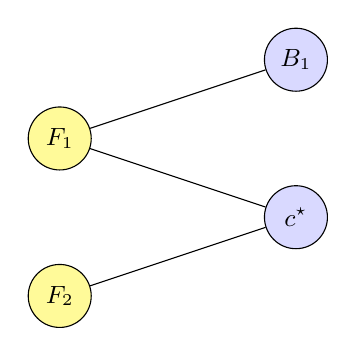
\begin{tikzpicture}[every node/.style={draw, circle, minimum size=8mm, inner sep=1pt, font=\small}]
  \node[fill=yellow!40] (F1) at (0,1) {$F_1$};
  \node[fill=yellow!40] (F2) at (0,-1) {$F_2$};
  \node[fill=blue!15] (B0) at (3,0) {$c^\star$};
  \node[fill=blue!15] (B1) at (3,2) {$B_1$};
  \draw (F1) -- (B0);
  \draw (F1) -- (B1);
  \draw (F2) -- (B0);
\end{tikzpicture}
\caption{Grafo de componentes de un ejemplo con dos componentes de primer plano.
$F_1$ tiene un agujero ($B_1$) y $F_2$ no, así que $\beta_0(F)=2$ y
$\beta_1(F)=(2-1)+(1-1)=1$. Ilustración propia.}
\label{fig:grafo-componentes}
\end{figure}

\paragraph{Grafo combinado~\cite[§2.1]{lux2025}.} Superponiendo $P$ y $G$, el plano se cubre con
cuatro regiones: verdaderos positivos (TP), verdaderos negativos (TN),
falsos positivos (FP) y falsos negativos (FN). Para evitar problemas de
conectividad en los bordes, se engrosa ligeramente el primer plano con
$\varepsilon$ y $2\varepsilon$. Las componentes conexas de las cuatro
regiones son los vértices del \emph{grafo combinado} $\mathcal{G}(P,G)$, con
aristas entre regiones adyacentes. Es bipartito: las aristas unen siempre
una región correcta (TP o TN) con una errónea (FP o FN).

\paragraph{Vértices regulares y críticos~\cite[§2.2--2.3]{lux2025}.} Un vértice erróneo
$v\in V_F$ es \emph{regular} si tiene exactamente un vecino TP y
exactamente un vecino TN:
\[
  V_r=\{v\in V_F : \exists!\,s\in N(v),\ s\subseteq\mathrm{TP}\ \wedge\
                  \exists!\,t\in N(v),\ t\subseteq\mathrm{TN}\}.
\]
Corregir un vértice regular solo desplaza una frontera y no cambia la
topología, así que su error es irrelevante para la forma. Los vértices
\emph{críticos} son el resto, $V_c=V_F\setminus V_r$, y la pérdida se
concentra en ellos:
\[
  \mathcal{L}_{CG}=\alpha\sum_{v\in V_c}\bar y_v,
\]
donde $\bar y_v$ es la probabilidad media de la clase predicha en los
píxeles de $v$. A diferencia de Betti matching, el gradiente actúa sobre
\emph{todos} los píxeles de cada región crítica.

\begin{proposicion}[{\cite[Prop.~2.1]{lux2025}}]
Si $\mathcal{L}_{CG}(P,G)=0$, todas las inclusiones del diagrama
\[
  F_\varepsilon(P)\ \hookleftarrow\ F_\varepsilon(P)\cap F_{2\varepsilon}(G)
  \ \hookrightarrow\ F_{2\varepsilon}(G),\qquad
  F_\varepsilon(P),\,F_{2\varepsilon}(G)\ \hookrightarrow\
  F_\varepsilon(P)\cup F_{2\varepsilon}(G)
\]
son retractos por deformación y, en particular, equivalencias homotópicas.
\end{proposicion}

Esta garantía es más fuerte que la del Betti matching. Las equivalencias
homotópicas inducen isomorfismos en homología, de modo que
$\mathcal{L}_{CG}=0$ implica $\tau^{\mathrm{err}}=0$. Además, Topograph
compara la unión con la \emph{intersección}, y no solo predicción y
referencia con su unión.

\paragraph{Métrica DIU~\cite[§2.5]{lux2025}.} La \emph{discrepancia entre intersección y
unión} usa la aplicación inducida por la inclusión
$i:F_\varepsilon(P)\cap F_{2\varepsilon}(G)\hookrightarrow
F_\varepsilon(P)\cup F_{2\varepsilon}(G)$:
\[
  \xi^{\mathrm{err}}=\dim\ker i_*+\dim\operatorname{coker} i_*.
\]
Por dualidad de Alexander, los agujeros del primer plano se corresponden
con componentes del fondo. Si $j$ es la inclusión análoga para los fondos,
\[
  \xi^{\mathrm{err}}=\dim\ker i_0+\dim\operatorname{coker} i_0
                    +\dim\ker j_0+\dim\operatorname{coker} j_0,
\]
de modo que basta contar componentes conexas. Intuitivamente, el
conúcleo cuenta componentes de la unión sin contrapartida en la
intersección y el núcleo cuenta componentes de la intersección que en la
unión se funden en una sola.

\paragraph{Complejidad~\cite[§2.6]{lux2025}.} Construir $\mathcal{G}(P,G)$ requiere etiquetar
componentes conexas, lo que con \emph{union-find} cuesta
$O(n\,\alpha(n))$. Como el grafo es plano, tiene $O(n)$ aristas, y
clasificar los vértices es lineal. Es la misma estructura que hace eficiente
el cálculo de $\operatorname{Dgm}_0$
(Sección~\ref{sec:persistencia-eficiente}), pero sin necesidad de ordenar
una filtración.

\subsection{Comparación}

La Tabla~\ref{tab:comparacion-topo} resume las diferencias entre los
enfoques descritos. Las pérdidas basadas en solapamiento de esqueletos, como
clDice~\cite{shit2021}, son eficientes y adecuadas para estructuras
tubulares, pero no ofrecen garantías topológicas formales.

\begin{table}[ht]
\centering
\small
\begin{tabular}{@{}lccc@{}}
\toprule
 & Hu et al.~\cite{hu2019} & BM~\cite{stucki2023} & Topograph~\cite{lux2025}\\
\midrule
Herramienta & persistencia & emp.\ inducidos & grafo de comp.\\
Correspondencia esp. & no & sí & sí\\
Usa la intersección & no & no & sí\\
Soporte del gradiente & 2 px/caract. & 2 px/caract. & regiones críticas\\
Coste & alto & alto & $O(n\,\alpha(n))$\\
Métrica asociada & --- & $\tau^{\mathrm{err}}$ & $\xi^{\mathrm{err}}$ (DIU)\\
\bottomrule
\end{tabular}
\caption{Comparación de los métodos topológicos para segmentación.}
\label{tab:comparacion-topo}
\end{table}
